\documentclass[prl,twocolumn]{revtex4-1}

\usepackage{graphicx}
\usepackage{color}
\usepackage{latexsym,amsmath}
\usepackage{physics}
\usepackage{hyperref}
\usepackage{subfig}
\definecolor{linkcolor}{rgb}{0,0,0.65} %hyperlink
\usepackage[pdftex,colorlinks=true, pdfstartview=FitV, linkcolor= linkcolor, citecolor= linkcolor, urlcolor= linkcolor, hyperindex=true,hyperfigures=true]{hyperref} %hyperlink%
\usepackage[backend=biber, sorting=ynt]{biblatex}
\usepackage{ragged2e} % to justify caption
\addbibresource{bibliography.bib}
\usepackage{tabularx}

\usepackage{fancyhdr}
\pagestyle{fancyplain}% <- use fancyplain instead fancy
\fancyhf{}
\fancyhead[R]{\thepage}
\renewcommand{\headrulewidth}{0pt}

\begin{document}

\title{EARTHQUAKES -- DBSCAN and t-SNE}

\author{Michele Guadagnini}
\author{Alessandro Lambertini}
\author{Alice Pagano}
\author{Michele Puppin}

\date{\today}

\begin{abstract}
Pattern recognition is a key learning task and clustering methods are one of the most powerful implementations for this aim.
Moreover, data visualization techniques are needed to analyze data with several features, which can be challenging for learning algorithms.
This work presents DBSCAN clustering method for unsupervised learning and t-SNE method for data visualization. After a theoretical overview of the two algorithms, we test their performances using a 5-dimensional labeled dataset with three embedded manifolds.

\end{abstract}

\maketitle
%%%%%%%%%%%%%%%%%%%%%%%%%%%%%%%%%%%%%%
\section{Introduction}
Machine Learning techniques describe how to learn a model that captures meaningful information from the data. In Unsupervised Learning no labels are given to the learning algorithm, leaving it on its own to find structure in its input.
Clustering methods are the simplest and most widely used implementations to achieve this aim. Clustering consists in grouping a set of objects according to some analogies such as the density distribution of the data points.
In Density-Based Clustering, clusters are regions of data space with higher density of data points separated from each other by contiguous regions of low point density.  The data points in the separating regions of low point density are typically considered noise or outliers \cite{Mehta_2019}\cite{doi:10.1002/widm.30}.

One realization of DB Clustering is DBSCAN, or Density Based Spatial Clustering of Applications with Noise, which requires two parameters. The parameter $\varepsilon$-neighborhood defines the radius of neighborhood around each data point, while the parameter \textit{minPts} is the minimum number of neighbors within $\varepsilon$ radius.
DBSCAN algorithm analyzes each point on a given dataset and classify them in three main categories. Any point in the dataset, with a neighbor count greater than or equal to \textit{minPts}, is marked as a \textit{core point}.
If the number of its neighbors is less than \textit{minPts}, but it belongs to the $\pmb{\varepsilon}$-neighborhood of another core point, it is marked as \textit{border point}. Finally, if a point is neither a core nor a border point, then it is called a noise point or an \textit{outlier}.
Moreover, a data point \(x_i\) is said to be \textit{density reachable} from another data point \(x_j\) if there is a path of core points leading from \(x_j\) to \(x_i\). Thus a cluster is defined as a group of density reachable points.
The main advantage of DBSCAN, or Density-Based clustering in general, is its capability of discovering clusters with arbitrary shapes. In addition, the computational complexity of efficient implementations of DBSCAN can achieve \(O(N \ln{N})\), where \(N\) is the length of the dataset
\cite{Mehta_2019}\cite{10.5555/3001460.3001507}.

Often large amount of data with several features are provided and data complexity can be challenging for learning algorithms. However, real data lay in a much lower dimensional space than the original space since in reality they are not uniformly distributed.
Furthermore, in order to choose the best predictive model one has to take into account the geometry and distribution of the data \cite{Mehta_2019}.

Therefore, data visualization methods are  introduced to reduce data complexity and to improve the understanding of data structure.
Dimensionality reduction is performed to project the data from the \textit{original space} onto a lower dimensional space, which is called the \textit{latent space}. Specifically, t-stochastic neighbor embedding (t-SNE) is a technique for dimensionality reduction which preserves the dataset local structure and it is particularly well suited for the visualization of high-dimensional datasets.
The core point is to associate to each data point a Gaussian probability distribution for its neighborhood.
The latter is defined as a symmetrized and normalized distribution \(p_{ij} \equiv (p_{i|j}+p_{j|i})/(2N) \) where
\begin{equation}
    p_{i|j} = \frac{\exp (- \norm{x_i-x_j}^2/2 \sigma ^2_i ) }
    { \sum_{k \neq i}^{} \exp (- \norm{x_i-x_k}^2/2 \sigma ^2_i ) }
\end{equation}
which provides an high probability for nearby points.
The symmetrization ensures that \( \sum_j p_{ij} > 1/(2N) \) for all data points, as a result of which each data point makes a significant contribution to the cost function which will be defined below.
Moreover, there is not an optimal value of the variance \( \sigma_i \) for all data points: a smaller value of \( \sigma_i \) is suited for points in high density regions. This is ensured by fixing the value of the local entropy \( H(p_i) \equiv -\sum_j p_{j|i} \log_2 p_{j|i}\) equal to \( \log_2{\Sigma}\), where \(\Sigma\) is called \textit{perplexity}. This is equivalent to imposing that all points have the same amount of information.
In the latent space an analogous, but long-tail, probability distribution is associated to each embedded data point. It is defined as
\begin{equation}
    q_{ij} = \frac{\qty(1 + \norm{y_i-y_j}^2)^{-1}  }
    { \sum_{k \neq i}^{} \qty(1 + \norm{y_i-y_k}^2)^{-1} }.
\end{equation}
The long-tail shape ensures that short distance information are preserved while far-away points are mapped to relatively large distances.
The aim of t-SNE is to find a low-dimensional data representation that minimizes the mismatch between \(p_{ij}\) and \(q_{ji}\). This is achieved by minimizing the cost function given by the Kullback-Leibler divergence between the distributions in the original and latent space:
\begin{equation}
    \mathcal{C}(Y)= D_{KL} (p||q) \equiv \sum_{ij} p_{ij} \log          \qty(\frac{p_{ij}}{q_{ij}}).
\end{equation}
Gradient descent is used for minimizing the cost function and the gradient results
\begin{equation}
    \partial_{y_i} \mathcal{C} =
    \sum_{j\neq i} 4 p_{ij} q_{ij} Z_i (y_i - y_j) - \sum_{j\neq i} 4 q_{ij}^2 Z_i (y_i-y_j)
\end{equation}
where \( Z_i = 1/(\sum_{k\neq i} (1+ \norm{y_k - y_i}^2 )^{-1}) \). Note that the minimization via gradient descent produces a stochastic algorithm. Moreover, t-SNE can produce equivalent result by rotating data and can deform scales in the latent space.
Eventually, it is a computationally intensive algorithm with a complexity of \(O(N^2)\) \cite{Mehta_2019}\cite{vanDerMaaten2008}.

%%%%%%%%%%%%%%%%%%%%%%%%%%%%%%%%%%%%%%
\section{Methods}
In this work we analyze a dataset containing three embedded manifolds with a linear closed structure in a 5-dimensional space as represented in Fig.~\ref{fig:3drep}. We use pre-labeled data for the aim of testing the performances of DBSCAN and t-SNE.

\begin{figure}[!t]
    \begin{minipage}[l]{1.0\columnwidth}
        \includegraphics[width=1.0\textwidth]{images/xrd/scattering_intensity.pdf}
        \caption{\justifying Representation of the manifolds using only the first three dimensions of the original space. Different colors are used to discern the three manifolds. \par}
        \label{fig:3drep}
    \end{minipage}
\end{figure}

%DBSCAN
In order to discern the three clusters, we use DBSCAN algorithm of the \textit{scikit-learn} library \cite{sk:dbscan} on the rescaled 5-dimensional dataset. A similar, but more noisy, dataset is tested as well.
To make the algorithm work properly, meaningful values of the parameters $\varepsilon$ and \textit{minPts} are needed. First of all, we choose \(\ln(N)\) as optimal value of \textit{minPts} where \(N\) is the number of data \cite{heuristic}.
Then, we compute the distances between each point and its \(k\) nearest neighbours, where \(k\) is equal to \textit{minPts}. In Fig.~\ref{fig:kdist} we plot an histogram of the distances: the greater value at which the tail of the histogram ends defines our $\varepsilon$ parameter. Indeed, this value in the histogram represents a change in density distribution among points. Eventually we tune the obtained parameters by setting up a grid of values.
Since the data labels are provided, the performance of DBSCAN is evaluated using the Normalized Mutual Information (NMI)  that measures the fraction of correctly predicted labels \cite{Mehta_2019}.

\begin{figure}[!t]
    \begin{minipage}[l]{1.0\columnwidth}
        \includegraphics[width=1.0\textwidth]{images/kdist.eps}
        \caption{\justifying Histogram of distances between each point and its \(k\) nearest neighbours. \par}
        \label{fig:kdist}
    \end{minipage}
\end{figure}

%t-SNE
We use t-SNE algorithm to represent the rescaled original data in a 2-dimensional \textit{latent space} using the algorithm implementation of the \textit{scikit-learn} library \cite{sk:tsne}. We test several values of the perplexity parameter \(\Sigma\) in order to compare results. Moreover, both the default random initialization and PCA initialization of the algorithm are tested.

% DBSCAN on t-SNE
Afterwards, we apply DBSCAN method to the dataset projected to the 2-dimensional \textit{latent space} with t-SNE algorithm.

\begin{figure*}[!tb]
  \centering
  \begin{minipage}[l]{1.0\textwidth}
   \subfloat[][]{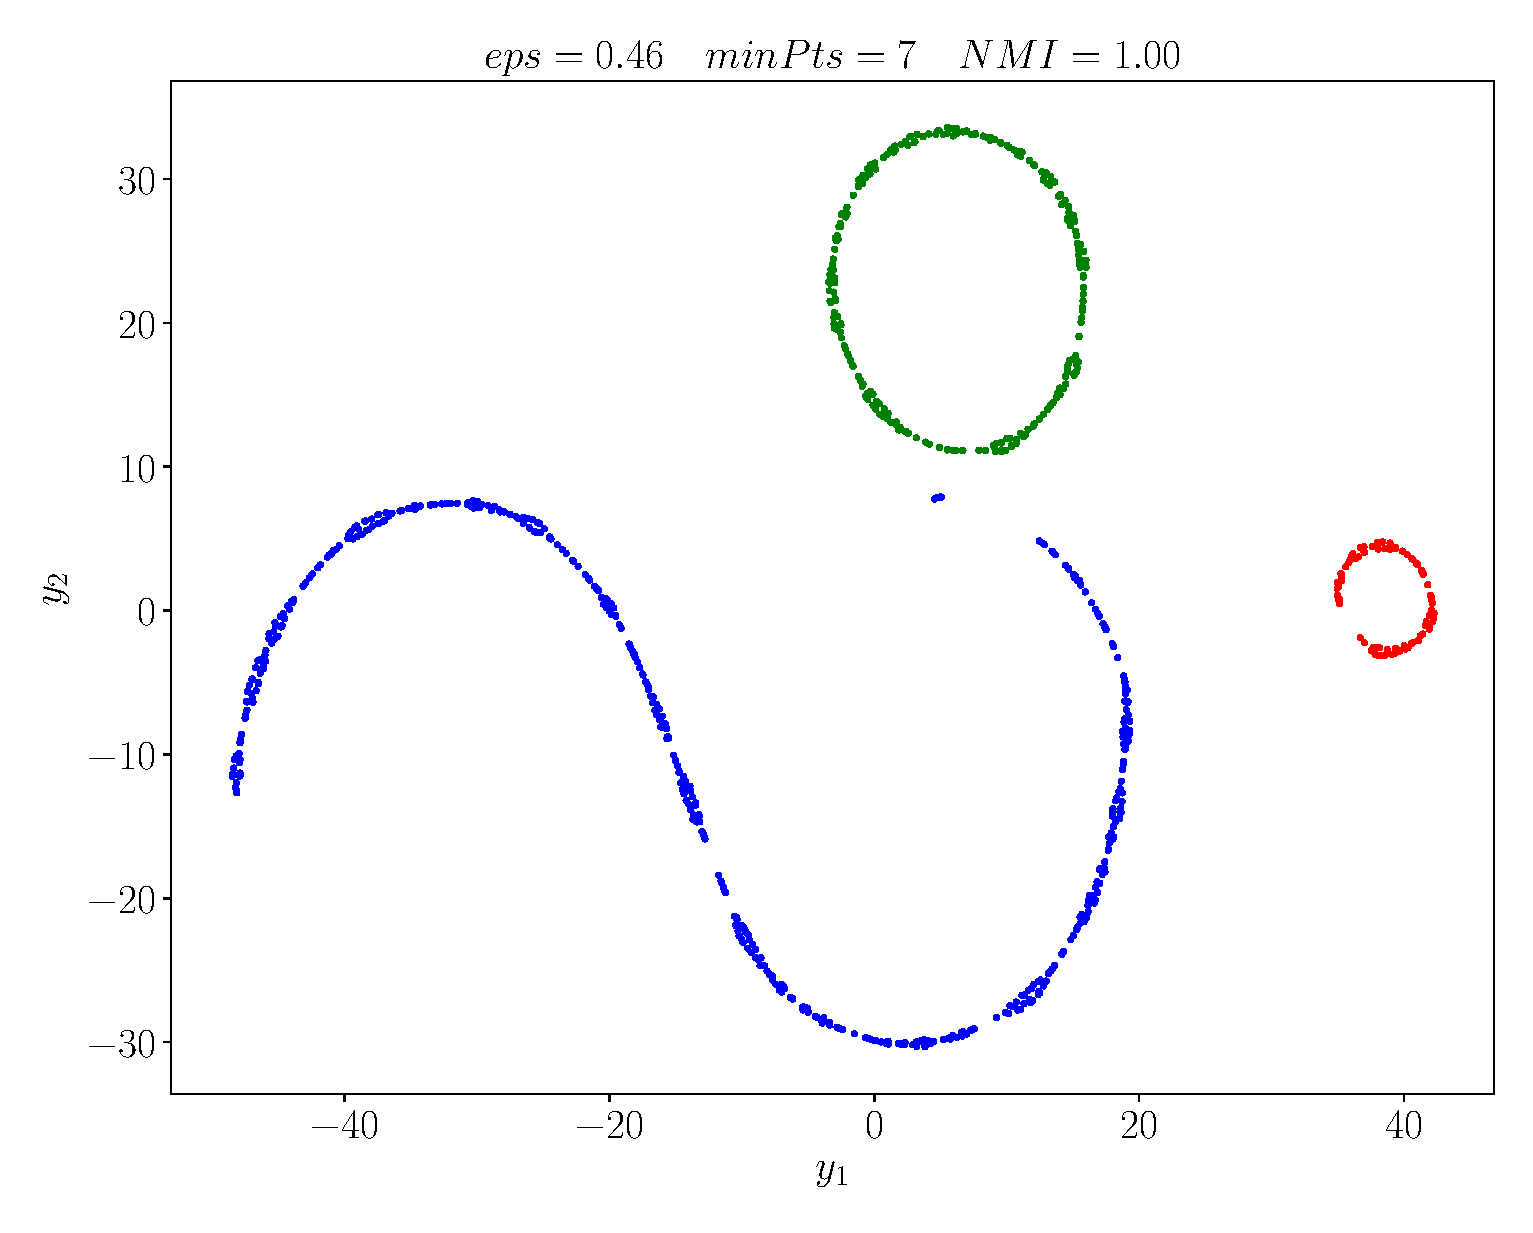
\includegraphics[width=0.49\textwidth]{images/dbscan5dim.eps}
  \label{fig:dbscan5dim} }
  \hskip 0.1cm
  \subfloat[][]{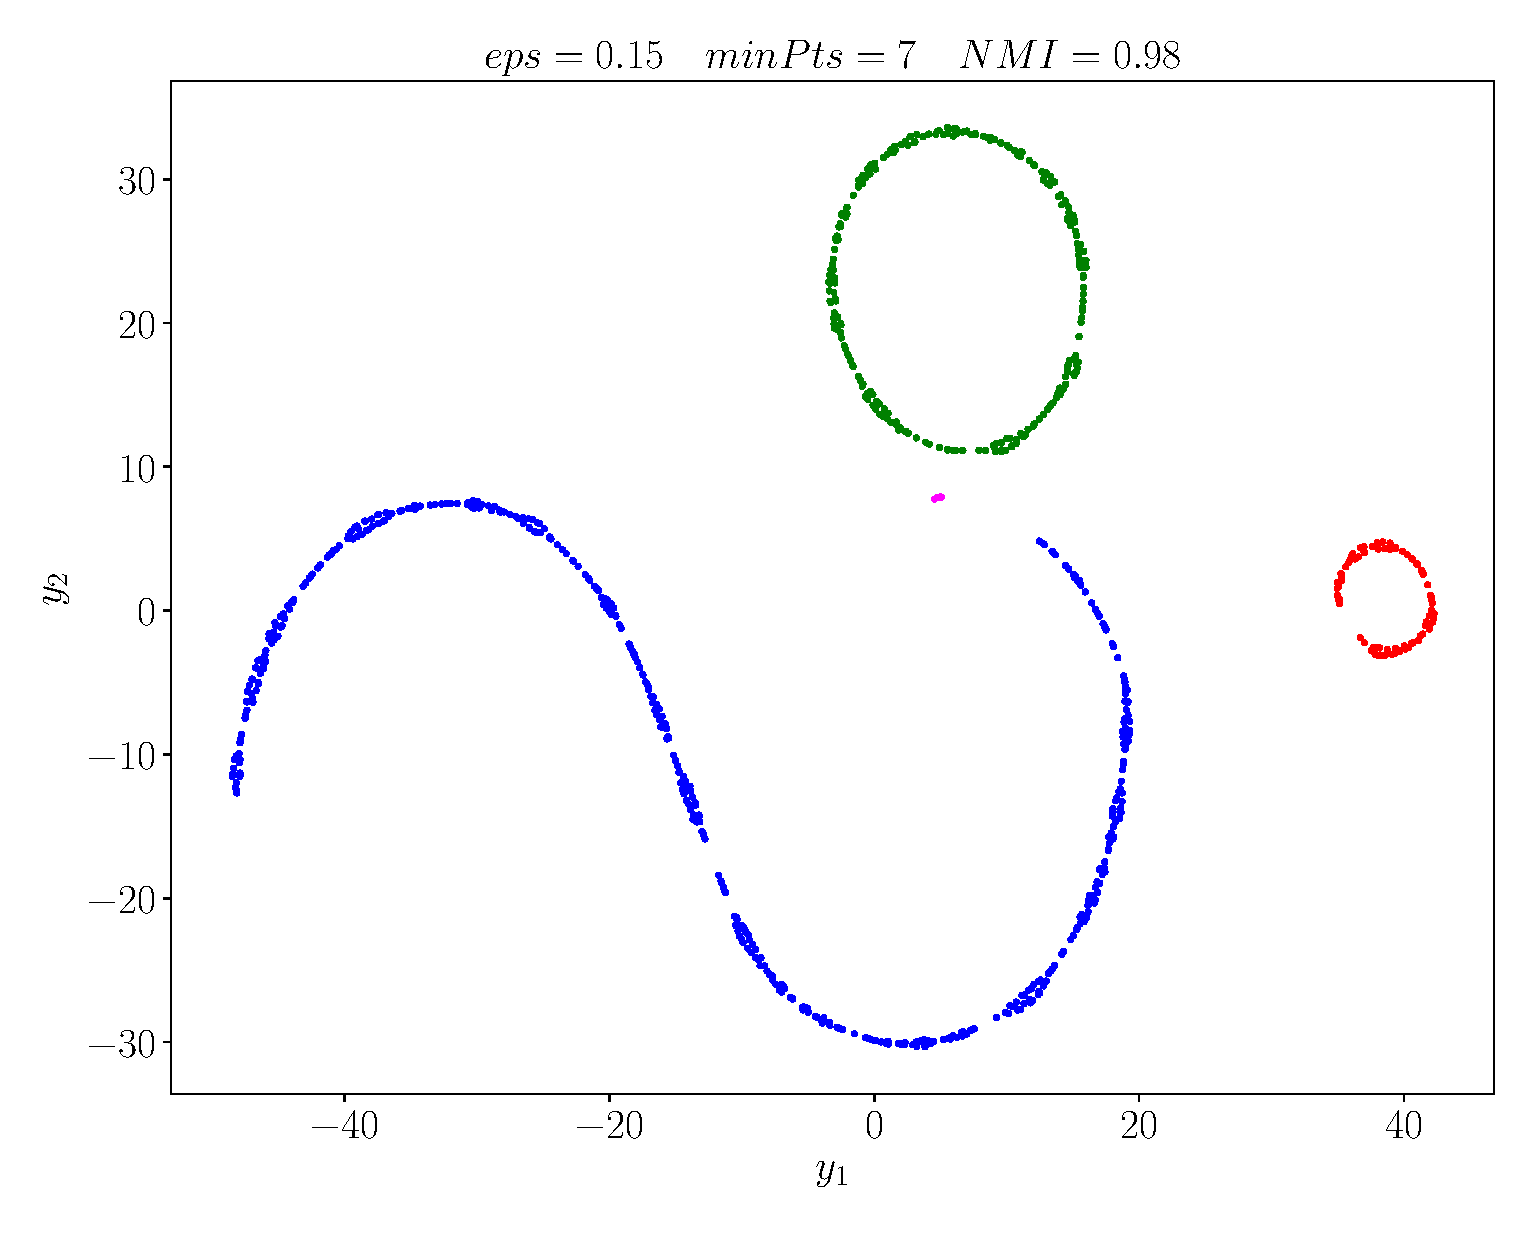
\includegraphics[width=0.49\textwidth]{images/dbscan2dim.eps}
  \label{fig:tsne_dbscan} }
  \vskip -0.27cm
  \subfloat[][]{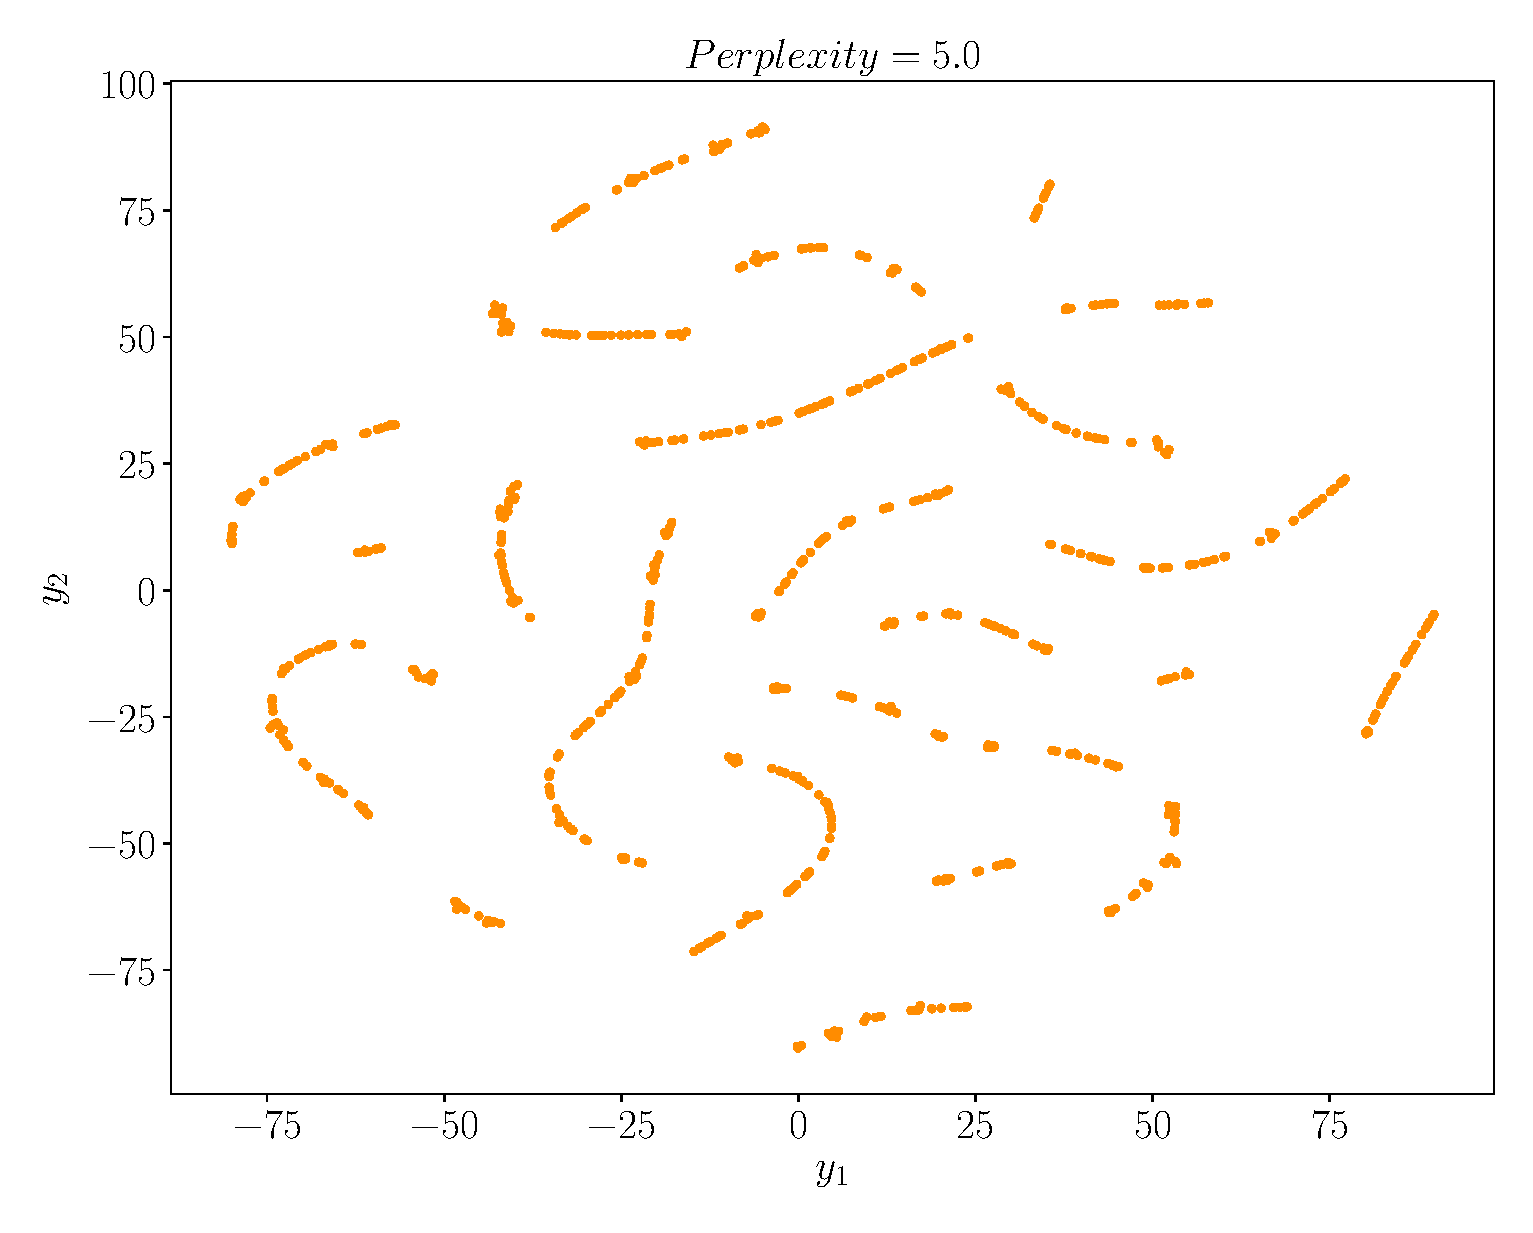
\includegraphics[width=0.49\textwidth]{images/perp1.eps}
  \label{fig:perp1} }
  \hskip 0.1cm
   \subfloat[][]{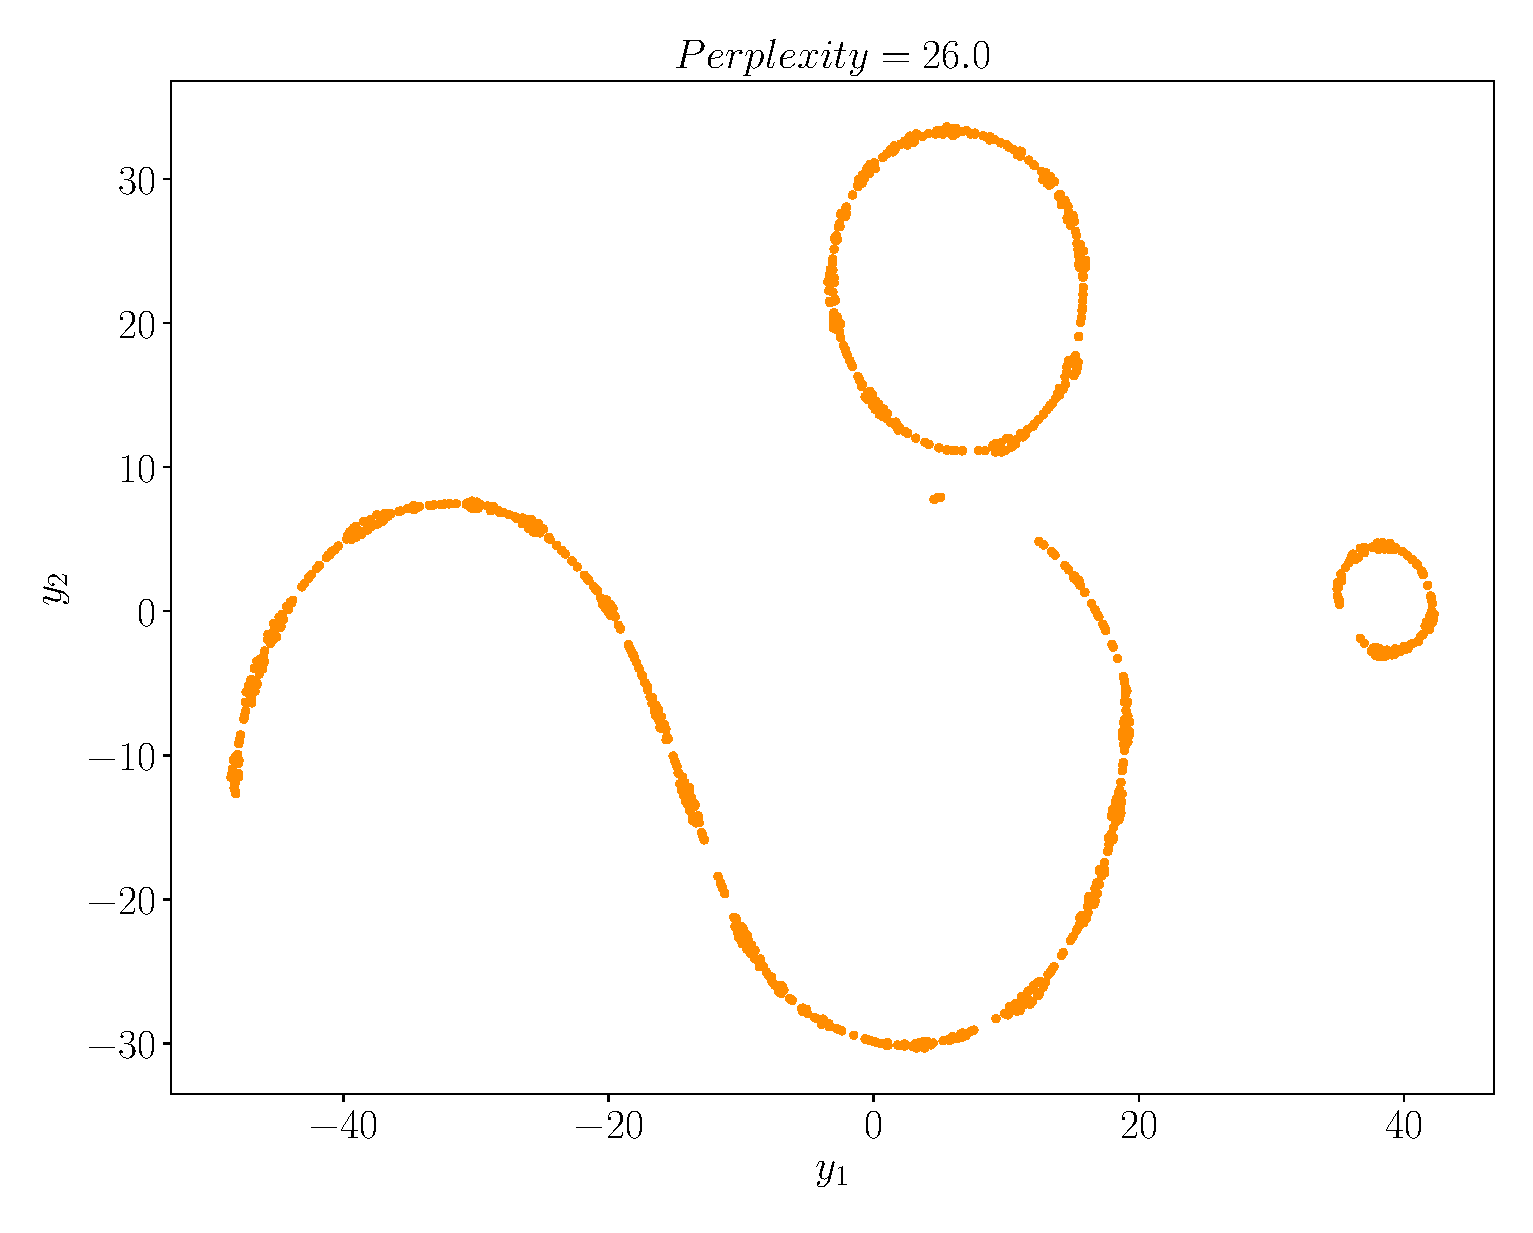
\includegraphics[width=0.49\textwidth]{images/perp2.eps}
   \label{fig:perp2} }
    \vskip -0.27cm
  \caption{ \justifying In (a) and (b) we plot the clustered manifold obtained by DBSCAN method on the 5-dim and 2-dim dataset respectively; for better visualization both are represented on the 2-dimensional \textit{latent space}. The three clusters are colored in blue, red and green, while outliers in magenta.
   In (c) and (d) we illustrate the dataset projected to the 2-dimensional \textit{latent space} with t-SNE for perplexity \(\Sigma = 5\)
   and \(\Sigma = 26\) respectively. \par }
  \label{fig:x}
  \end{minipage}
\end{figure*}

%%%%%%%%%%%%%%%%%%%%%%%%%%%%%%%%%%%%%%
\section{Results}
For DBSCAN method on the 5-dimensional dataset we set the value of the parameter \textit{minPts}\(=7\) and \(\varepsilon=0.46\). We illustrate the results for a grid of the parameters \textit{minPts} and \(\varepsilon\) in Table~\ref{tab:1}. Several combination of the parameters return a NMI of 1.00 and we choose \textit{minPts}\(=7\) and \(\varepsilon=0.46\) as best parameters since they are the expected ones.

\begin{table}[h!]

\begin{minipage}[l]{1.0\columnwidth}
\centering

\begin{tabular*}{\columnwidth}{@{\extracolsep{\fill}}lccccccccc}
%\colrule
\multicolumn{10}{c}{\textbf{\textit{minPts} = 7}}  \\
\colrule
\(\pmb{\varepsilon} \) & 0.38 & 0.40 & 0.42 & 0.44 & 0.46 & 0.48 & 0.50 & 0.52 & 0.54 \\
 \textbf{NMI}          & 0.81 & 0.98 & 0.98 & {\color{blue}1.00} & {\color{blue}1.00} & {\color{blue}1.00} & {\color{blue}1.00} & {\color{blue}1.00} & 0.00  \\
\colrule
&&&&&&&&& \\
%\colrule
\multicolumn{10}{c}{\(\pmb{\varepsilon=0.46} \)}  \\
\colrule
\textbf{\textit{minPts}} & 3    & 4    & 5    & 6    & 7    & 8    & 9    & 10   & 11 \\
 \textbf{NMI}            & {\color{blue}1.00} & {\color{blue}1.00} & {\color{blue}1.00} & {\color{blue}1.00} & {\color{blue}1.00} & {\color{blue}1.00} & 0.81 & 0.72 & 0.70  \\
\colrule
\end{tabular*}

\caption{\justifying NMI results for grid of \textit{minPts} and \(\varepsilon\) values for DBSCAN in 5-dim dataset. \par}
\label{tab:1}
\end{minipage}
\vspace{-0.7cm}

\end{table}


In Fig.~\ref{fig:dbscan5dim} the results are plotted on the 2-dimensional dataset obtained with t-SNE for better visualization. We observe that the three clusters are thoroughly labeled, indeed we compute a
value of NMI equal to 1.


Then, in Fig.~\ref{fig:perp1} and Fig.~\ref{fig:perp2} we visualize the dataset projected to the 2-dimensional \textit{latent space} with t-SNE with random initialization for perplexity \(\Sigma = 5, 26\) respectively. For \(\Sigma = 5\) the algorithm is not able to project the data in a meaningful way, while for \(\Sigma = 26\) we can see that the structure of the three clusters is preserved. Moreover, we verify that PCA initialization does not produce sensibly different results.

In Fig.~\ref{fig:tsne_dbscan} we apply DBSCAN method on the 2-dimensional dataset. After the grid search we obtain that best performance are achieved for \textit{minPts}\(=7\) and \(\varepsilon=0.15\). We observe that the three clusters are not thoroughly labeled, indeed we compute a value of NMI equal to 0.98. We note that t-SNE projects badly the overlapping part of two clusters labeling it as an outlier.

Eventually, we reproduce the same analysis on a more noisy dataset. We observe that DBSCAN method has lower performances and require higher value of \textit{minPts}. Moreover, the noise challenges t-SNE making it harder to discern the overlapping parts of the clusters.

%%%%%%%%%%%%%%%%%%%%%%%%%%%%%%%%%%%%%%
\section{Conclusions}
In this  work, we show that DBSCAN on the 5-dimensional dataset with three embedded manifolds is able to discern clusters correctly. In particular, the method we choose for selecting \textit{minPts} and \(\varepsilon\) parameters proves to be very effective.
Moreover, we show that t-SNE is able to project meaningfully the dataset in a 2-dimensional \textit{latent space} for proper value of the perplexity parameter.
However, the loss of information in the projected \textit{latent space} challenges DBSCAN making it misclassify some overlapping points as outliers.
%Thus it is more convenient to use t-SNE when a dataset with a large number of features is provided.
Eventually, we observe that with more noisy dataset performance is generally reduced.


\printbibliography

\end{document}
